% !TEX root = main.tex
\renewcommand{\labelenumi}{\alph{enumi})}
\section*{Semanal 5}
\textbf{1. Sea $\Sigma$ = \{a, b\}, 
disena un AFN que reconozca el mismo lenguaje que contiene
combinaciones de subcadenas 'aa' o 'aab' y todas terminan en b.}


\textbf{1. Sea $\Sigma$ = \{a, b, c\}, 
disena un AFN-$\epsilon$ que acepte todas las cadenas que contengan exactamente
dos simbolos distintos del alfabeto.}

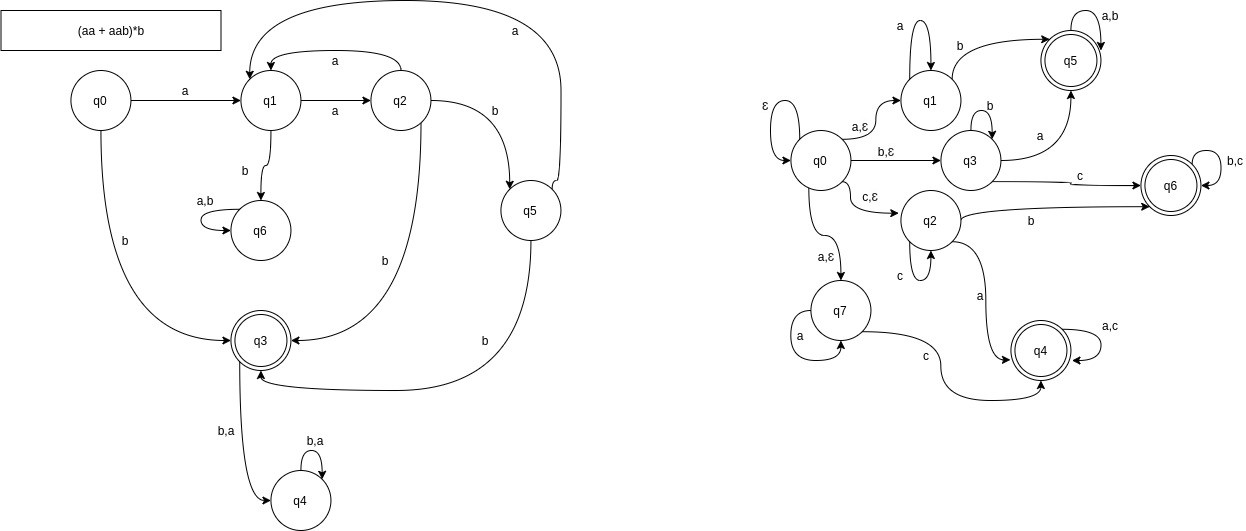
\includegraphics[scale=.70]{semanal5.jpg}
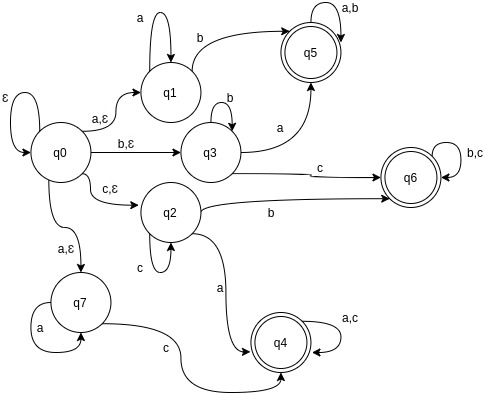
\includegraphics[scale=.70]{semanal5 (1).jpg}
